%-------------------------------------------------------------------------------
\section{Approximate Solution}\label{Approximation}
%------------------------------------------------------
Even in this simplified model, the evaluation of $E\max$ at all states creates a considerable computational burden. As alternative parameterizations are appraised during an estimation, it requires the repeated evaluation of a four-dimensional integral by Monte Carlo integration at a total of 163,410 states. Building on the idea of generalized polynomial approximation \citep{Bellman.1963}, \citet{Keane.1994} propose to calculate $E\max$ only at a subset of states each period and interpolate its value for the rest. Their key choices are the interpolation function and the number of interpolation points. I will now describe their approach in detail, successfully recompute their original quality diagnostics, and provide some additional insights that underscore the trade-off between computation time and the accuracy of estimation results. I follow \citet{Keane.1994} in all the details of the analysis that follows unless otherwise noted. Additional results and implementation details are available in Appendix \ref{Results}.
%-------------------------------------------------------------------------------
\subsection{Operationalization}
%-------------------------------------------------------------------------------
After experimentation, \citet{Keane.1994} settle on equation (\ref{Interpolation Function}) as their preferred interpolation function.
%
\begin{align}\label{Interpolation Function}
E \max - \max E = \pi_0 + \sum^4_{j = 1} \pi_{1j} (\max E - \bar{V}_j) +
\sum^4_{j = 1} \pi_{2j} \left(\max E - \bar{V}_j\right)^{\tfrac{1}{2}}
\end{align}
%
$\bar{V}_j$ is shorthand for the expected value of the alternative-specific value function and $\max E = \max_k\{\bar{V}_j\}$ is its maximum among the choices available to the agent. The $\pi$'s are time-varying as they are estimated by ordinary least squares period by period. The subset of interpolation points used to fit the interpolating function, i.e. where $E\max$ is calculated explicitly, is chosen at random for each period. The number of interpolation points remains constant across all periods.\\\newline
%
My implementation of the backward induction procedure remains straightforward. Period by period, I determine whether the total number of states is larger than the number of interpolation points. If this is not the case, $E\max$ is evaluated at each state. Otherwise, I draw a random sample of states for the interpolation points, evaluate $E\max$ and fit equation (\ref{Interpolation Function}). Based on the results, I construct the predicted values for all remaining states in that period. Applying this interpolation scheme with 200 interpolation points reduces the number of states at which $E\max$ is explicitly evaluated from 163,410 to 6,930 which cuts the computation time for each evaluation of the criterion function to about a twentieth.
%-------------------------------------------------------------------------------
\subsection{Quality Diagnostics}
%-------------------------------------------------------------------------------
Within the general setup of equation (\ref{Interpolation Function}), \citet{Keane.1994} carefully analyze the impact of alternative tuning parameters such as the number of interpolation points and the number of random draws for the evaluation of $E\max$ integral on the reliability of results. They generate three Monte Carlo samples with different parameterizations of the reward functions. I focus on their first parameterization in the text but all other results are available in the Appendix.\\\newline
%
To assess the quality of the proposed interpolation scheme, I use an \textit{exact solution} of the model as a benchmark. This solution is computed using 100,000 random draws for the evaluation of $E\max$ at all states at the true parameter values. The \textit{exact sample} refers to a set of 1,000 simulated agents based on the \textit{exact solution}. As on overall measure of the approximation error, I use the root-mean-square error (RMSE) and compare the choice probabilities in the \textit{exact sample} to the results from a newly simulated set of 1,000 agents based on the alternative parameterization of the model.
%-------------------------------------------------------------------------------
\paragraph{Simulation based on Approximate Solution.}
%-------------------------------------------------------------------------------
Table \ref{Paper: Correct Choices} shows the proportion of correct choices for alternative interpolation schemes. I vary the number of interpolation points and the number of random draws for the evaluation of $E\max$. I follow each agent in the \textit{exact sample} over time and evaluate for each period whether a choice based on an approximate solution is still correct, i.e. aligns with the choice based on the \textit{exact solution}. If I evaluate $E\max$ at all states with 2,000 random draws, then the two choices align for 96\% of the agents in the sample in all 40 periods. This share drops to 75\% as I only use 200 states each period and interpolate the rest. While always remaining above 39 periods, the average number of correct choices for each agent decreases as I coarsen the approximation.
\begin{table}\onehalfspacing
\begin{center}
\begin{threeparttable}
  \captionsetup{width=30cm}
  \caption{Correct Choices}
  \label{Paper: Correct Choices}
  \begin{tabular}{lrrrrr}\toprule
  Points     & All & All & All   & 2000 & 500   \\
  $E\max$ Draws & 2000 & 1000 & 250 & 2000 & 2000  \\
  \midrule
  Periods & \mc{5}{c}{} \\
  \phantom{0}1 - 10  &   0.000 &  0.000 &  0.000 &  0.000 &  0.000 \\
  11 - 35            &   0.000 &  0.000 &  0.000 &  0.000 &  0.000 \\
  36 - 38            &   0.010 &  0.000 &  0.020 &  0.027 &  0.046 \\
  39                 &   0.036 &  0.043 &  0.181 &  0.190 &  0.252 \\
  40                 &   0.963 &  0.957 &  0.799 &  0.783 &  0.702 \\
  Average            &  39.962 & 39.957 & 39.777 & 39.752 & 39.649 \\
    \bottomrule
  \end{tabular}
\end{threeparttable}
\end{center}
\end{table}

%-------------------------------------------------------------------------------
\paragraph{Estimation based on Approximate Solution.}
%-------------------------------------------------------------------------------
To assess the impact of the approximation as it ripples through an estimation, I perform a Monte Carlo exercise by sampling a subset of 100 agents forty times from the \textit{exact sample}. Starting each  bootstrap iteration from the true parameter values, I evaluate the criterion function based on an approximate solution to the DP problem using 200 interpolation points and 500 random draws for the evaluation of $E\max$. On average the optimizer stops after 880 function evaluations and 196 steps. The RMSE remains small with about 0.03 when simulating a new sample based on the mean parameter values across all bootstrap iterations. \\\newline
%
So far I successfully recomputed the diagnostics provided in \citet{Keane.1994} and the results are encouraging. However, given the experience in \citet{Eisenhauer.2015b}, I worry that the approximation error introduces noise in the criterion function resulting in many local minima. If so, a Monte Carlo exercise that uses the true parameters as the starting values potentially disguises the trade-off between computation time and reliability of results as the optimizer simply gets stuck in a local minimum close by. To assess the validity of my concern, I will now investigate the noise in the criterion function and conduct a more challenging version of the Monte Carlo exercise.
%-------------------------------------------------------------------------------
\paragraph{Noise in Criterion Function.}
%-------------------------------------------------------------------------------
In Figure \ref{Criterion Functions}, I trace out the exact and the approximate criterion function from the previous Monte Carlo exercise around the true parameter values. To get a sense of the discrepancy between the two, I perturb $\beta_1$, which captures the tuition cost of a higher education, around its true value in \$100 increments. For comparison, I normalize both functions to zero at the minimum of the exact function. While the exact criterion function has its minimum at the actual value this is not true for for the approximated function. The latter attains its minimum at a perturbation of -\$100. This casts doubt on the quality of the approximation.
\begin{figure}[h!]
\caption{Criterion Functions}\label{Criterion Functions}
\centering
\scalebox{0.30}{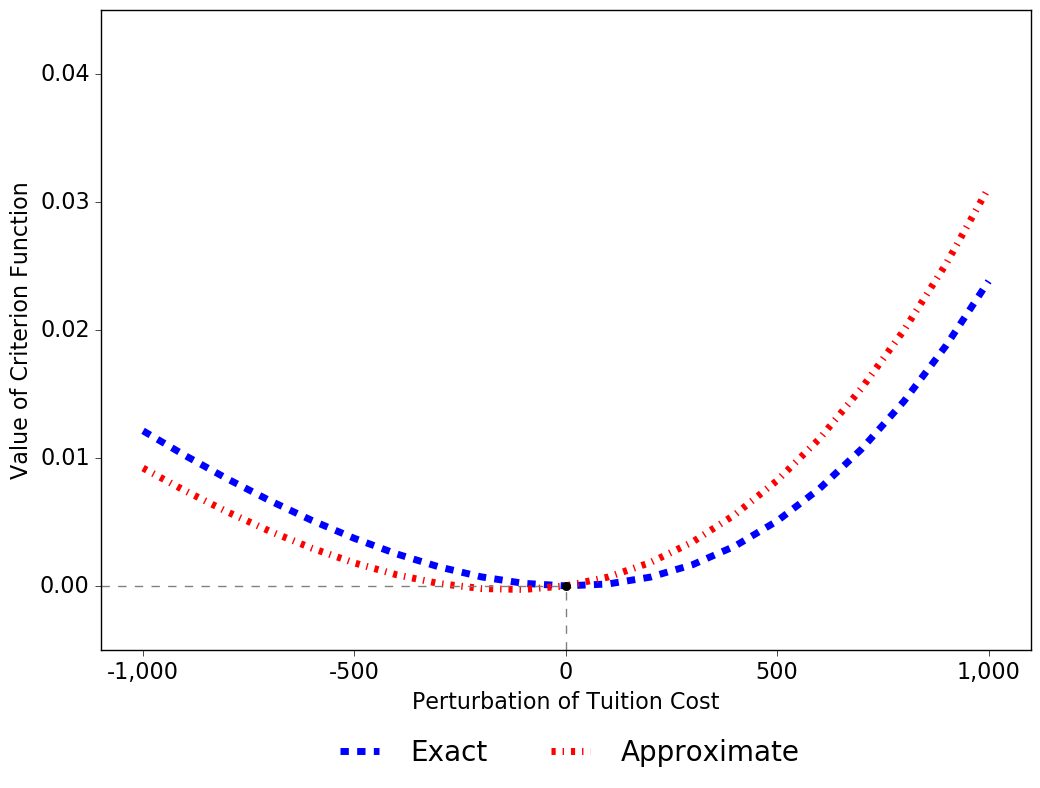
\includegraphics{../material/graph_criterions.png}}\vspace{0.5cm}
\end{figure}

%-------------------------------------------------------------------------------
\paragraph{Estimation based on Approximate Solution (revisited).}
%-------------------------------------------------------------------------------
I thus conduct a slightly modified version of the previous Monte Carlo exercise by choosing more challenging starting values. I first estimate a misspecified static model $(\delta = 0.00)$ starting from the true parameterization of the dynamic model using the \textit{exact sample}. I then use the estimation results as starting values for the subsequent estimation of a correctly specified dynamic model $(\delta = 0.95)$ on the same dataset. Table \ref{Interpolation Schemes} summarizes the results for alternative interpolation schemes. Focusing on the RMSE and the total computation time in minutes, it shows how the accuracy of results increases with the refinement of the interpolation scheme. However, this comes at the cost of steep increases in computation time.
\begin{table}\onehalfspacing
\begin{center}
\begin{threeparttable}
  \captionsetup{width=30cm}
  \caption{Interpolation Schemes}
  \label{Interpolation Schemes}
  \begin{tabular}{lrrrr}\toprule
  Points      & 200 & 500 & 1,500  & All \\
  $E\max$ Draws & 500 &  500 &   500 & 500 \\
  \midrule
  RMSE        & 0.10 &   0.09 &    0.07 &  0.03  \\
  Minutes     &  35 &      96 &    361 &   794 \\
  Steps       &  1,090 &   2,671 &   5,730 &  32,774 \\
  Evaluations & 3,017 &   6,412 &    12,020 & 59,680 \\ %why steps and evals switched in old?
  \bottomrule
  \end{tabular}\scriptsize
  \begin{tablenotes}\item \textbf{Notes:} All results are calculated as the average across all 40 Monte Carlo iterations.
  \end{tablenotes}
  \end{threeparttable}
  \end{center}
\end{table}

